% This is "sig-alternate.tex" V2.1 April 2013
% This file should be compiled with V2.5 of "sig-alternate.cls" May 2012
%
% This example file demonstrates the use of the 'sig-alternate.cls'
% V2.5 LaTeX2e document class file. It is for those submitting
% articles to ACM Conference Proceedings WHO DO NOT WISH TO
% STRICTLY ADHERE TO THE SIGS (PUBS-BOARD-ENDORSED) STYLE.
% The 'sig-alternate.cls' file will produce a similar-looking,
% albeit, 'tighter' paper resulting in, invariably, fewer pages.
%
%--------------------------
% This .tex file (and associated .cls V2.5) produces:
%       1) The Permission Statement
%       2) The Conference (location) Info information
%       3) The Copyright Line with ACM data
%       4) NO page numbers
%
% as against the acm_proc_article-sp.cls file which
% DOES NOT produce 1) thru' 3) above.
%
% Using 'sig-alternate.cls' you have control, however, from within
% the source .tex file, over both the CopyrightYear
% (defaulted to 200X) and the ACM Copyright Data
% (defaulted to X-XXXXX-XX-X/XX/XX).
% e.g.
% \CopyrightYear{2007} will cause 2007 to appear in the copyright line.
% \crdata{0-12345-67-8/90/12} will cause 0-12345-67-8/90/12 to appear in the copyright line.
%
% ---------------------------------------------------------------------------
% This .tex source is an example which *does* use
% the .bib file (from which the .bbl file % is produced).
% REMEMBER HOWEVER: After having produced the .bbl file,
% and prior to final submission, you *NEED* to 'insert'
% your .bbl file into your source .tex file so as to provide
% ONE 'self-contained' source file.
%
% ================= IF YOU HAVE QUESTIONS =======================
% Questions regarding the SIGS styles, SIGS policies and
% procedures, Conferences etc. should be sent to
% Adrienne Griscti (griscti@acm.org)
%
% Technical questions _only_ to
% Gerald Murray (murray@hq.acm.org)
% ===============================================================
%
% For tracking purposes - this is V2.0 - May 2012

\documentclass{sig-alternate-05-2015}

%\usepackage{tabu}
%\usepackage{multirow}

\usepackage{booktabs}


\begin{document}

% Copyright
\setcopyright{acmcopyright}
%\setcopyright{acmlicensed}
%\setcopyright{rightsretained}
%\setcopyright{usgov}
%\setcopyright{usgovmixed}
%\setcopyright{cagov}
%\setcopyright{cagovmixed}

\clubpenalty=10000
\widowpenalty = 10000


%Conference
\conferenceinfo{GECCO'16,} {July 20-24, 2016, Denver, Colorado, USA.}

% \acmPrice{\$15.00}

%
% --- Author Metadata here ---
\CopyrightYear{2016} % Allows default copyright year (20XX) to be over-ridden - IF NEED BE.
\crdata{TBA}  % Allows default copyright data (0-89791-88-6/97/05) to be over-ridden - IF NEED BE.
% --- End of Author Metadata ---

%\title{Parent Selection and Diversification in Genetic Programming}

%\title{Error Diversity in Lexicase and Tournament Selection}

\title{Effects of Lexicase and Tournament Selection on Diversity Recovery and Maintenance}

%
% You need the command \numberofauthors to handle the 'placement
% and alignment' of the authors beneath the title.
%
% For aesthetic reasons, we recommend 'three authors at a time'
% i.e. three 'name/affiliation blocks' be placed beneath the title.
%
% NOTE: You are NOT restricted in how many 'rows' of
% "name/affiliations" may appear. We just ask that you restrict
% the number of 'columns' to three.
%
% Because of the available 'opening page real-estate'
% we ask you to refrain from putting more than six authors
% (two rows with three columns) beneath the article title.
% More than six makes the first-page appear very cluttered indeed.
%
% Use the \alignauthor commands to handle the names
% and affiliations for an 'aesthetic maximum' of six authors.
% Add names, affiliations, addresses for
% the seventh etc. author(s) as the argument for the
% \additionalauthors command.
% These 'additional authors' will be output/set for you
% without further effort on your part as the last section in
% the body of your article BEFORE References or any Appendices.

\numberofauthors{3} %  in this sample file, there are a *total*
% of EIGHT authors. SIX appear on the 'first-page' (for formatting
% reasons) and the remaining two appear in the \additionalauthors section.
%
\author{
% 1st. author
\alignauthor
Thomas Helmuth\\
       \affaddr{Computer Science}\\
       \affaddr{Washington and Lee U.}\\
       \affaddr{Lexington, Virginia, USA}\\
       \email{helmutht@wlu.edu}
% 2nd. author
\alignauthor
Nicholas Freitag McPhee\\
       \affaddr{Div. of Science \& Mathematics}\\
       \affaddr{U. of Minnesota, Morris}\\
       \affaddr{Morris, Minnesota, USA}\\
       \email{mcphee@morris.umn.edu}
% 3rd. author
\alignauthor Lee Spector\\
       \affaddr{Cognitive Science}\\
       \affaddr{Hampshire College}\\
       \affaddr{Amherst, Massacusetts, USA}\\
       \email{lspector@hampshire.edu}
}

\maketitle
\begin{abstract}
In genetic programming systems, parent selection algorithms select the programs from which offspring will be produced by random variation and recombination. While most parent selection algorithms select programs on the basis of aggregate performance on multiple test cases, the lexicase selection algorithm considers each test case individually, in random order, for each parent selection event. Prior work has shown that lexicase selection can produce both more diverse populations and more solutions when applied to several hard problems. Here we examine the effects of lexicase selection, compared to those of the more traditional tournament selection algorithm, on population error diversity using two program synthesis problems. We conduct experiments in which the same initial population is used to start multiple runs, each using a different random number seed. The initial populations are extracted from genetic programming runs, and fall into three categories: high diversity populations, low diversity populations, and populations that occur after diversity crashes. The reported data shows that lexicase selection can maintain high error diversity and also that it can re-diversify less-diverse populations, while tournament selection consistently produces lower diversity.
\end{abstract}

%
%  Use this command to print the description
%
\printccsdesc

% We no longer use \terms command
%\terms{Theory}

\keywords{diversity, lexicase selection, tournament selection, hyperselection, PushGP}

\section{Introduction}
\label{sec:introduction}

Parent selection is one of the fundamental processes in genetic programming (GP), and several different parent selection algorithms have been developed. Lexicase selection is a relative newcomer on the scene \cite{Spector:2012:GECCOcompANEW, Helmuth:2015:ieeeTEC}. While most commonly-used parent selection algorithms, such as tournament selection, select programs on the basis of aggregate performance on multiple test cases, the lexicase selection algorithm considers each test case individually, in random order, for each parent selection event. 
Compared to tournament selection, lexicase selection has been shown to produce more diverse populations and more solutions on several classes of problems, including software synthesis benchmark problems \cite{Helmuth:2015:ieeeTEC, Helmuth:2015:dissertation, Helmuth:2015:GECCO, Helmuth:2015:GPTP}. This prior work made connections between high diversity and high solution rates when using lexicase selection. Each of these studies examined the diversity of entire GP runs, each starting with a different initial population and random number seed.

Our work here was originally motivated by observations of dramatic drops in diversity that result from ``hyperselection'' events when using lexicase selection, in which one or a few individuals in the population receive the majority of the parent selections in a generation \cite{Helmuth:2016:GECCO}. Anecdotally, these runs often seemed to recover diversity within a handful of generations following the diversity crash. Because a capability for recovering adaptive diversity is desirable, we decided to examine the dynamics of diversity  after diversity crashes more systematically, producing data from runs using lexicase selection and, for comparison, tournament selection. 

While examining the effects of selection algorithms in the wake of diversity crashes is enlightening, such a study has scope limited to infrequent events when using lexicase selection. More broadly, we are interested in the immediate effects on diversity that these algorithms have in populations with other defining characteristics. In particular, we wish to explore how each method influences diversity in populations that occur naturally during evolution, specifically in populations with usually high or low diversity.

In order to study these questions, we conducted sets of runs in which each run was initialized with the same population, with each population extracted from a GP run. This allows us to observe how different selection methods affect diversity when started on the exact same population.

In the next section we describe the two selection algorithms in our study. We then describe our experimental design, including a discussion of the diversity measure that we used (error diversity), the ways in which we extracted initialization populations, the two test problems that we used, and the parameters of our runs. Finally, we present the results of the experiments and discuss their implications.


\section{Parent Selection}

In this section we describe the two parent selection algorithms used in our experiments.

\subsection{Tournament Selection}

We use standard tournament selection as a comparison method. In it, we choose random individuals (with replacement) to form a tournament set, and select the individual with the lowest total error to be a parent.

%{\it General description.}
%
%{\it Maybe tournament size for tournaments in this paper given here, with pointers to papers studying multiple tournament sizes.}

\subsection{Lexicase Selection}

Each time a parent must be selected, lexicase selection first shuffles the list of test cases into a random order. Then, starting with the entire population, it removes any individual that did not achieve the best error value on the first test case. As long as more than one individual remains in the population, the first test case is removed and this process is repeated with the next test case, etc. For each test case, any individual that did not have the \textit{best} error of \textit{those remaining in the pool} is removed from consideration. If at any point only a single individual remains, it is selected as the winner of that parent selection event. On the other hand, if every test case is exhausted and multiple individuals remain, one of them is randomly selected. A more detailed description of lexicase selection is given in \cite{Helmuth:2015:ieeeTEC}.


Lexicase selection shares some motivation with other recent techniques that consider not how an individual performs across an entire problem in aggregate, but instead how it performs on parts of a problem. This work on ``behavior-based'' or ``semantic'' search operators includes geometric semantic GP \cite{Moraglio2012}, behavioral GP \cite{Krawiec:2014:GECCO}, clustering test cases into objectives \cite{Krawiec:2015:EuroGP, Krawiec:2015:GECCO:smgpWorkshop}, and other behavior-based search drivers \cite{Krawiec:2015:GPTP}. Lexicase selection sets itself apart from these methods by placing importance on individual test cases and combinations of test cases---those test cases that come at the beginning of each random ordering of cases.


\section{Experimental Design}

In this paper we concentrate on diversity measures related to the outputs of the programs. One such diversity measure, \textit{behavioral diversity}, has been shown to correlate with problem-solving performance \cite{Jackson:2010:PPSN}. In behavioral diversity, the output of a program on each training case input is recorded as a \textit{behavior vector}. Behavioral diversity is then the percentage of distinct behavior vectors in the population. \textit{Error diversity}, a slight variation of behavioral diversity, considers the percentage of distinct \textit{error vectors} in the population where each error vector is computed by applying the error function to each output in the behavior vector. We believe error diversity does a good job of measuring how well evolution is exploring meaningful differences between programs that might be lost with a diversity measure that only takes into account syntactic (genotypic) diversity of the population, since two wildly different programs may actually compute the same function.

In order to produce the populations on which to experiment, we started GP runs and let them continue until they met certain stopping conditions; we then stored those populations and later conducted multiple trials with different random number seeds starting with those stored populations. We used three different stopping conditions in order to generate naturally occuring populations with interesting properties:
\begin{itemize}
\item {\bf High diversity:}
In runs using lexicase selection, we stopped if the population error diversity was greater than 0.9. This produces  diverse populations, allowing us to observe whether evolution is able to maintain such high diversity in the following generations.

\item {\bf Low diversity:}
In runs using tournament selection, we stopped if the population error diversity was less than 0.15. These populations allow us to see if methods promote diversification starting from such undiverse populations.

\item {\bf After a diversity crash:}
As described above, we were initially motivated here by observations of runs using lexicase selection that underwent major drops in diversity following hyperselection events. In this condition, we stopped runs using lexicase selection when the error diversity reached a level at least 0.25 less than it had been at some point in the previous 10 generations. This allowed us to detect populations that had recently undergone large drops in diversity. We do not definitively know whether those drops are related to hyperselection events, but we expect that they are.

\end{itemize}
In all three conditions, we only considered populations occurring after the first 10 generations in order to give evolution a chance to settle down after the extreme shifts that can happen at the beginning of a run.

In each trial, we continued running GP on a stored population for 20 generations while recording the population error diversity. For each parent selection setting (lexicase and tournament selection), we conducted 100 trials with different random number seeds from the same stored population.

We conducted these tests on two problems taken from a recent program synthesis benchmark suite \cite{Helmuth:2015:GECCO}. The first problem, Replace Space With Newline (RSWN), requires the production of a program that takes a string as input and both prints an output string and returns a result. The printed string should be a copy of the input string with all spaces replaced by newline characters. The functionally returned result should be the number of non-whitespace characters in the input string. Previous examinations of error vector diversity on the RSWN problem show that lexicase selection maintains significantly higher diversity than tournament selection \cite{Helmuth:2015:GPTP}.

The second problem, Double Letters, requires the production of a program that takes a string as input and prints the string after doubling every alphabetic character and tripling every exclamation point. All other characters should be printed once. As with the RSWN problem, lexicase selection consistently achieves high diversity on this problem. Differently than RSWN, runs using tournament selection show slow but steady increases in diversity, though not approaching that of lexicase selection runs \cite{Helmuth:2015:GPTP}.

\begin{table}[t]
\centering
\caption{PushGP parameters}
\label{table:parameters}
%\rowcolors{3}{Gray}{white}
\begin{tabular}{l r}
\toprule
\textbf{Parameter} & \textbf{Value} \tabularnewline
\midrule
runs per problem/parent selection combination & 100 \tabularnewline
population size & 1000 \tabularnewline
maximum genome size & 800 \tabularnewline
maximum initial genome size & 400 \tabularnewline
%alternation rate & 0.01 \tabularnewline
%alignment deviation & 10 \tabularnewline
%uniform mutation rate & 0.01 \tabularnewline
%uniform close mutation rate & 0.1 \tabularnewline
tournament size (for tournament selection) & 7 \tabularnewline
\midrule
\end{tabular}
\begin{tabular}{l r}
\textbf{Genetic Operator} & \textbf{Probability} \tabularnewline
\midrule
alternation & 0.2 \tabularnewline
uniform mutation & 0.2 \tabularnewline
uniform close mutation & 0.1 \tabularnewline
alternation followed by uniform mutation & 0.5 \tabularnewline
\bottomrule
\end{tabular}
\end{table}

For our experiments we used PushGP \cite{spector:2002:GPEM, 1068292}, a stack-based GP system.\footnote{Lexicase selection has also been shown to be effective in tree-based GP \cite{Helmuth:2015:ieeeTEC, Krawiec:2015:GECCO:smgpWorkshop}.} PushGP supports a variety of control structures and multiple data types, making it a good choice for program synthesis tasks such as the problems we explore here.
Except for parent selection, we used the exact same PushGP parameters in both the initial runs used to store interesting populations as well as the continuations of the stored populations. We give the most relevant parameters in Table~\ref{table:parameters}. The parameters not listed here exactly follow those described in \cite{Helmuth:2015:dissertation}, where the meanings of all parameters are also explained in detail.

These runs use the most recent version of PushGP, in which individuals are stored as linear genomes that we translate into hierarchical Push programs prior to execution \cite{Helmuth:2015:dissertation}. These linear genomes admit a range of uniform genetic operators; we use four, listed in Table~\ref{table:parameters} with their probabilities. Alternation is a linear crossover operator modeled after the recombinative portion of ULTRA \cite{Spector:2013:GPTP}. Uniform mutation may replace each instruction with 1\% probability. Uniform close mutation may add or remove hierarchy-delineating parentheses from the program.
%\footnote{Opening parentheses are inserted during the translation from linear Plush genomes to structured Push programs, according to the code-block requirements of instructions, while closing parentheses are inserted where indicated by epigenetic ``close'' markers attached to genes; these markers are the targets of uniform close mutation.}
Finally, the last operator runs alternation on two parents and then uniform mutation on that child to produce a new child.


\section{Results}
\label{sec:results}

Using the techniques presented in the previous section we obtained populations on which to perform continuation experiments. For each combination of the two problems and three stopping conditions we stored populations from two runs, for a total of 12 populations. In the following subsections we group the results based on the stopping conditions, since they produce the most similar populations.
%Note that we label each population with a letter; these letters have no relation to the populations themselves, and are simply used for reference.

Starting with each stored population we conducted 100 ``continuation'' GP runs with lexicase selection and 100 with tournament selection. We let each continuation evolve for 20 generations, and plot the population error diversity across the runs. In particular, each figure has a standard box-and-whisker plot for each generation, with the box showing the median and quartiles. The whiskers stretch to the maximum and minimum values, ignoring outliers. In each figure we also plot the error diversity of each individual run at each generation, giving another way of visualizing the spread of diversities across runs.

Note that in a few settings, one or two runs out of 100 found solutions to the problem before the end of 20 generations. In these cases, we terminate the runs, and they do not contribute data past their termination generation.



\subsection{Starting with high diversity}
\label{sec:highDiversityResults}

First, we examine continuations initialized with populations that were evolved using lexicase selection and achieved error diversity greater than $0.9$. As such, the initial populations of the continuations have very high diversity, with most individuals producing distinct error vectors.

\begin{figure*}
	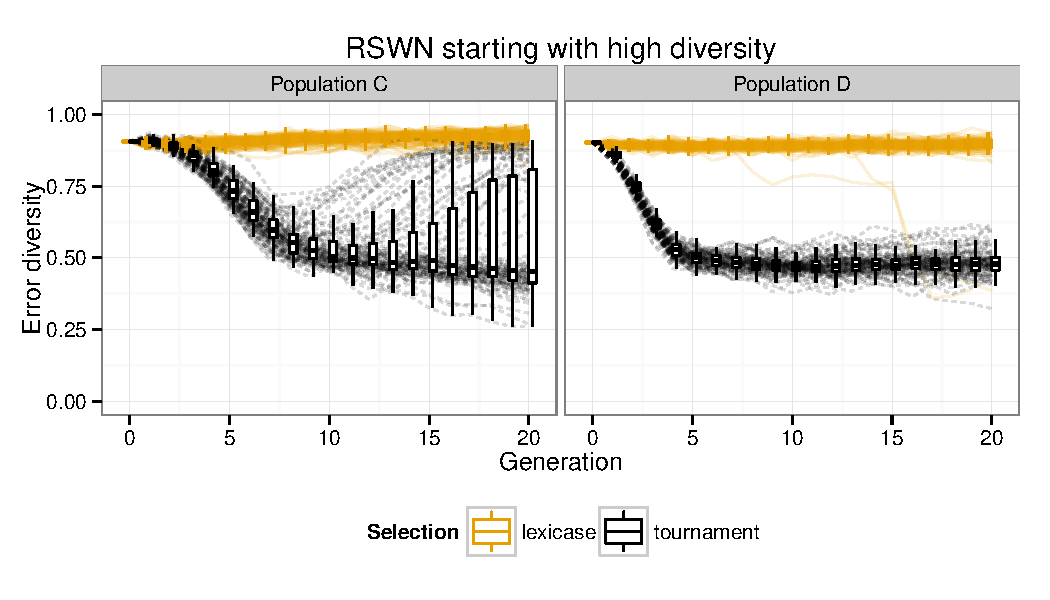
\includegraphics{../figures/RSWN_high_diversity}
	\vspace{-1 cm}
	\caption{Error diversity over 100 continuations of the RSWN problem with both lexicase and tournament selection, starting from populations with high diversity naturally occuring in a run using lexicase selection.}
	\label{fig:RSWNhighDiversity}
\end{figure*}

\begin{figure*}
	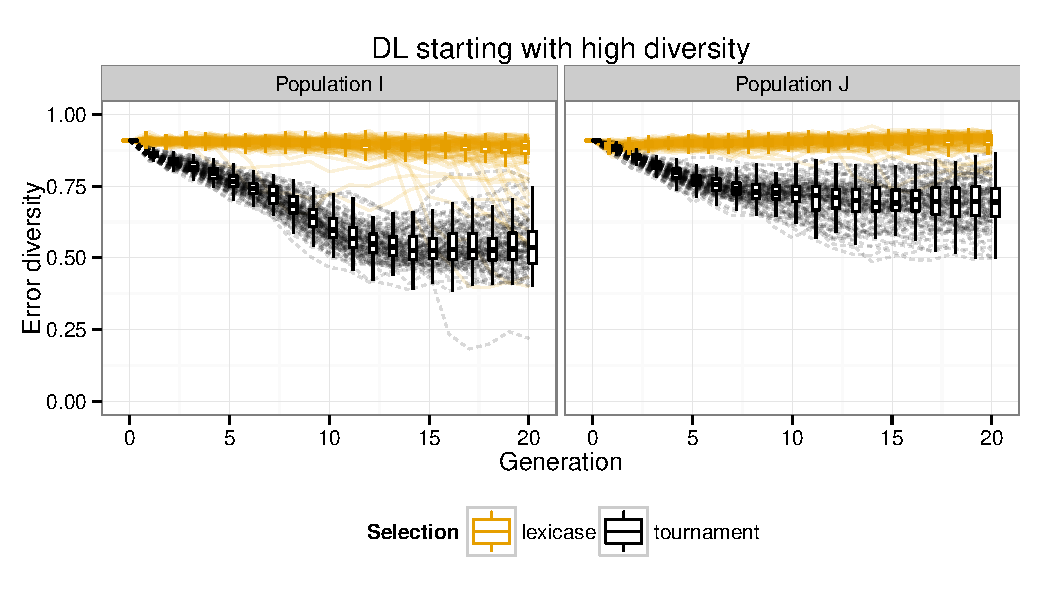
\includegraphics{../figures/DL_high_diversity}
	\vspace{-1 cm}
	\caption{Error diversity over 100 continuations of the double-letters problem with both lexicase and tournament selection, starting from populations with high diversity naturally occuring in a run using lexicase selection.}
	\label{fig:DLhighDiversity}
\end{figure*}

\begin{figure*}
	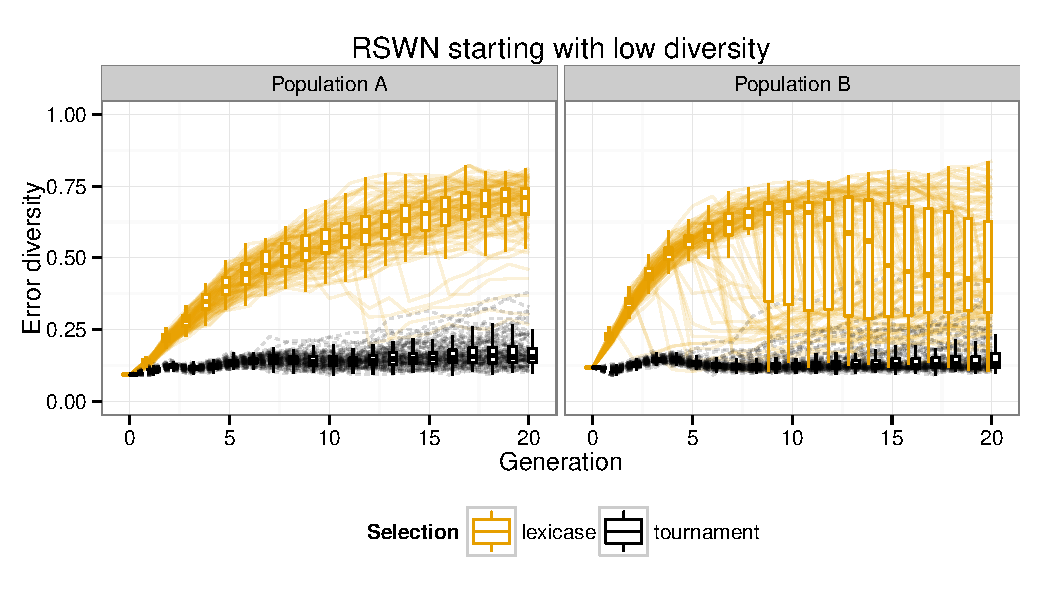
\includegraphics{../figures/RSWN_low_diversity}
	\vspace{-1 cm}
	\caption{Error diversity over 100 continuations of the RSWN problem with both lexicase and tournament selection, starting from populations with low diversity  naturally occuring in a run using tournament selection.}
	\label{fig:RSWNlowDiversity}
\end{figure*}

\begin{figure*}
	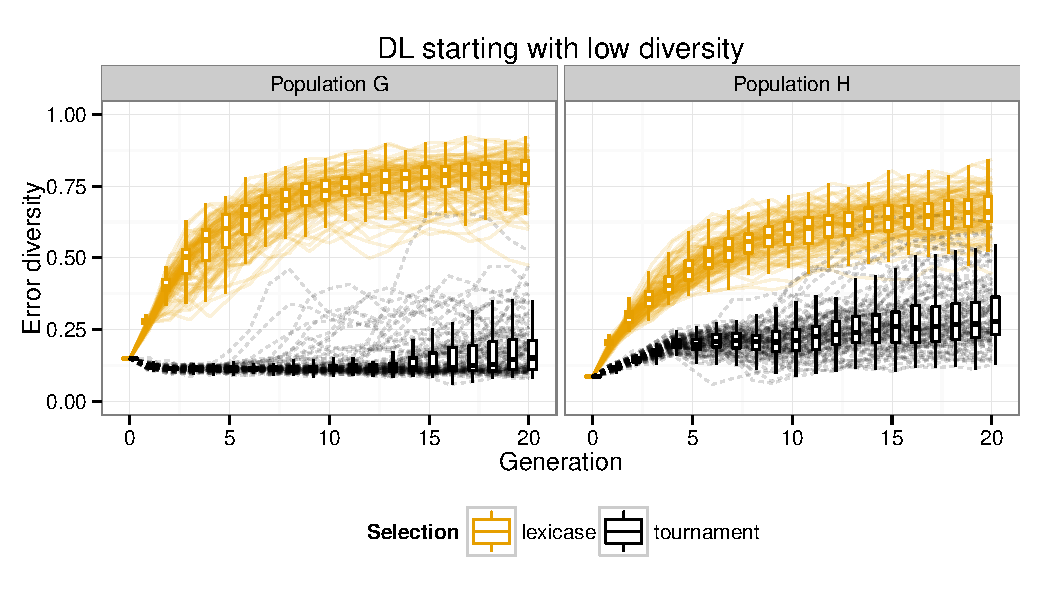
\includegraphics{../figures/DL_low_diversity}
	\vspace{-1 cm}
	\caption{Error diversity over 100 continuations of the double-letters problem with both lexicase and tournament selection, starting from populations with low diversity naturally occuring in a run using tournament selection.}
	\label{fig:DLlowDiversity}
\end{figure*}

\begin{figure*}
	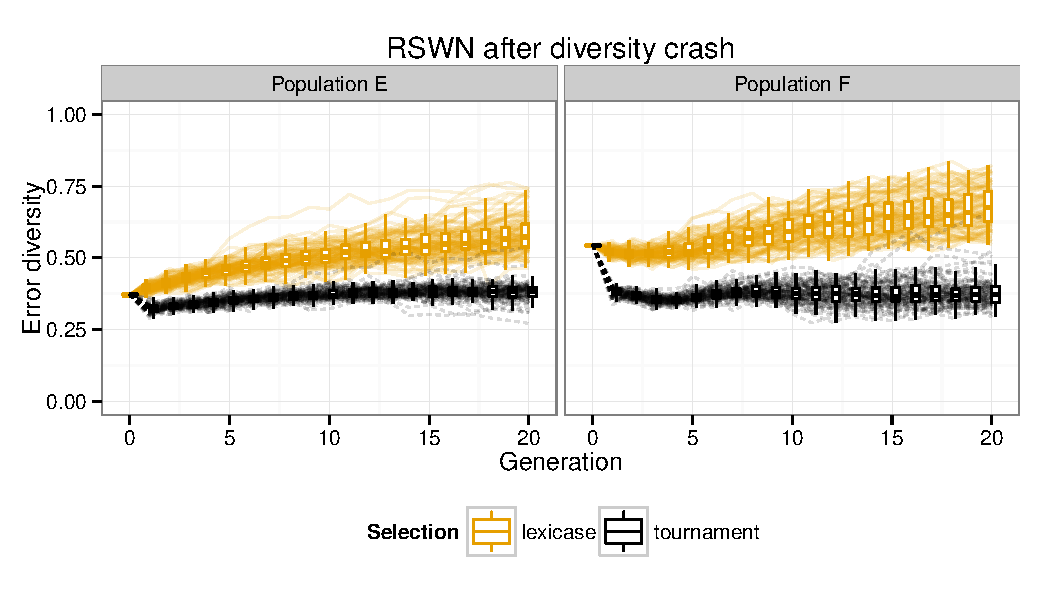
\includegraphics{../figures/RSWN_diversity_crash}
	\vspace{-1 cm}
	\caption{Error diversity over 100 continuations of the RSWN problem with both lexicase and tournament selection, starting from populations that had lost at least 25\% error diversity in a diversity crash in a lexicase selection run.}
	\label{fig:RSWNdiversityCrash}
\end{figure*}

\begin{figure*}
	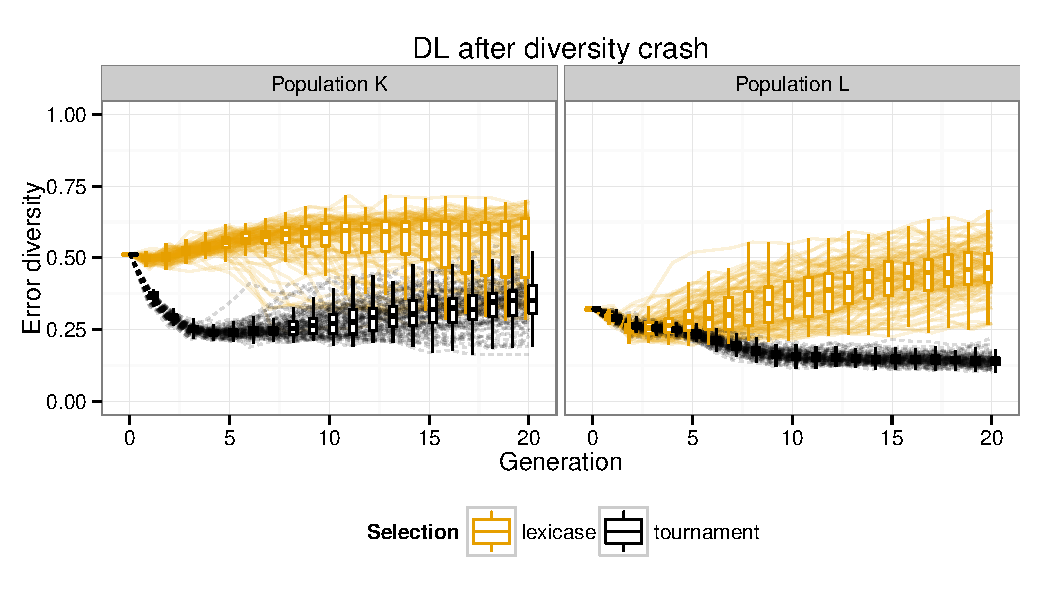
\includegraphics{../figures/DL_diversity_crash}
	\vspace{-1 cm}
	\caption{Error diversity over 100 continuations of the double-letters problem with both lexicase and tournament selection, starting from populations that had lost at least 25\% error diversity in a diversity crash in a lexicase selection run.}
	\label{fig:DLdiversityCrash}
\end{figure*}

Figure~\ref{fig:RSWNhighDiversity} plots the continued runs started from two populations (A and B) stored from GP on the RSWN problem. Lexicase selection consistently maintains high levels of diversity starting from both populations, with little variance. On the other hand, both plots show runs using tournament selection quickly losing significant diversity within the first 5 to 10 generations of the continuation, dropping from over 90\% distinct error vectors down to around 50\% distinct error vectors. Interestingly, the tournament selection runs on Population A show large differences in diversity in the last 10 generations, with some becoming even less diverse while others recover much of the lost diversity. On the other hand, the tournament selection runs on Population B maintain much more consistent diversity, with most runs having between 40\% and 60\% diversity in the remaining generations.
%It is unclear to us why these two populations result in such different diversity plots for tournament selection, but we assume it has to do with the composition of the stored population.

Figure~\ref{fig:DLhighDiversity}, which plots the diversities of continuations of two populations (C and D) on the Double Letters problem, shows similar trends in both lexicase selection and tournament selection. Note that tournament selection maintains higher diversity on this problem than on the RSWN problem, though not as high as lexicase selection. This trend mirrors what has been seen previously on full GP runs \cite{Helmuth:2015:GPTP}.


%Nic: Some of the individual drops in lexicase diversity are likely due to hyperselection events. Some of those then recovered, but it's not clear that all did; not sure what we say about that part.
%Tom: I wouldn't worry about it. Some runs that don't recover are pretty outliery to me.


\subsection{Starting with low diversity}
\label{sec:lowDiversityResults}

Next, we present continuations of runs that start from populations exhibiting very low population diversity, at most 0.15. In other words, most of the individuals in these populations produced the same error vectors. These populations were stored from runs that used tournament selection, since we were not able to achieve population diversity this low in a run using lexicase selection. Additionally, these runs will shed light on whether the parent selection technique used to produce the initial populations has effect on the continued diversity.

Figure~\ref{fig:RSWNlowDiversity} plots diversity of runs starting from populations E and F on the RSWN problem. Starting from both populations, tournament selection does not increase diversity across the 20 generations except for a handful of outlier runs. The continuations using lexicase selection increase the median diversity across runs rapidly, with over 50\% unique error vectors by generation 8 using population E and generation 4 using population F. For population E, lexicase selection runs continue to steadily rise in diversity over the 20 generations. On the other hand, many runs starting with population F undergo steep drops in diversity, such that by generation 9 the lower quartile of diversity falls precipitously from around 60\% to around 35\%. The indivdiually plotted run diversities show that many runs continue to see single-generation drops in diversity throughout the 20 generations. We believe this population likely contained one or more individuals that, when varied in the right way, produce a child that dominates the rest of the population, leading to hyperselection events---and therefore drops in diversity---in many runs. Even with these drops in diversity, lexicase selection maintains higher diversity than tournament selection in the majority of continuations.

We present continuations of low-diversity populations (G and H) evolved on the Double Letters problem in Figure~\ref{fig:DLlowDiversity}. Lexicase selection again increases error diversity more quickly than tournament selection, though here tournament selection does show some increases in diversity. This is more pronounced when starting from population H, where median diversity is over 0.25 by generation 20. This still pales in comparison to lexicase selection's diversity, which grows to more than 0.6 on population H and 0.75 on population G. Both plots show lexicase selection runs gaining and maintaining diversity across the 20 generations, without any of the diversity drop-offs that we observed in Figure~\ref{fig:RSWNlowDiversity}.


\subsection{Starting after a diversity crash}
\label{sec:crashDiversityResults}


In Figure~\ref{fig:RSWNdiversityCrash} we plot error diversity from populations I and J on the RSWN problem, which were stored after diversity crashes of at least 25\%.
For the lexicase selection runs, neither of these plots shows rapid rediversification; instead, we see consistent gains in diversity for most of each run.
The median diversity on population I increases about 20\% over 20 generations, gaining back most of the diversity it lost during the diversity crash. Population J gains back about 15\% population in that timespan.
Interestingly, population I sees immediate small gains in diversity in the first few generations, whereas population J shows consistent small losses in diversity before rediversifying. This presumably means that population I had reached its minimum in its diversity crash, whereas population J was recorded near the end of the crash but before its minimum.

Turning our attention to tournament selection, we see that it produced remarkably consistent drops in diversity in the very first generation, especially in Population J. These drops are followed by little movement either direction during the remaining generations.

Figure~\ref{fig:DLdiversityCrash} shows the same settings for the Double Letters problem using populations K and L. Population K is interesting in that lexicase selection gains some diversity near the beginning while almost every tournament selection loses at least 25\% diversity over the first 4 generations. After that, an increasing number of lexicase selection runs seem to undergo further diversity crashes, pulling down the lower quartile while the median diversity stays around 60\%. On the other hand, tournament selection shows incrases in diversity in the later generations, although its quartiles never overlap with lexicase selection's.

For population L, after a few generations of further diversity decreases, lexicase selection runs tend to increase diversity (with lots of variation) ending with about 20\% higher median diversity than at its lowest. Tournament selection, however, consistently loses diversity over the 20 generations with little variance across runs.

\section{Discussion}


The results from continuations of high-diversity populations clearly show that lexicase selection can maintain a high population diversity while tournament selection cannot reliably do so. One notable feature visible in the initial-high-diversity plots (Figure~\ref{fig:RSWNhighDiversity} and Figure~\ref{fig:DLhighDiversity}) is the occasional steep drop in diversity in a small number of runs using lexicase selection, which can be seen especially clearly in populations B and C. Based on similar runs we have encountered previously, we would guess that these runs underwent hyperselection events in which one or a small number of individuals were selected to make most of the children in a single generation. Hyperselection events can, understandably, lead to diversity crashes since most of the individuals in the population are closely related. Interestingly, previous work has shown that such events are neither a driving force nor a hinderance in runs using lexicase selection \cite{Helmuth:2016:GECCO}.

The continuations starting from low-diversity populations (Figures~\ref{fig:RSWNlowDiversity} and \ref{fig:DLlowDiversity}) show how lexicase selection can diversify an un-deriverse population over a small number of generations. This ability to create error diversity helps to explain how lexicase selection can rapidly explore the space of meaningfully different programs.


Of the results we present, those from runs starting with populations that were produced by diversity crashes (Figure~\ref{fig:RSWNdiversityCrash} and Figure~\ref{fig:DLdiversityCrash}) show the smallest gaps in diversity between lexicase selection and tournament selection. Still, they demonstrate lexicase selection's ability to increase diversity, albeit gradually, following a diversity crash. Tournament selection runs lost diversity over the 20 generations in three of the four conditions, showing not only that it was unable to stop the diversity crash, but also that it extended and exacerbated the crash.

In summary, the reported data shows that lexicase selection can maintain high error diversity and also that it can re-diversify less-diverse populations, whether those populations were produced by tournament selection or by diversity crashes with lexicase selection. Tournament selection consistently produced lower diversity, either by decreasing the number of unique error vectors in the population or by failing to increase diversity in un-diverse populations. 

The higher diversity seen with lexicase selection does not, for the problems and configurations examined here, come at the expense of problem-solving power---quite the contrary. In data reported elsewhere \cite{Helmuth:2015:GECCO}, lexicase selection produced solutions to the Replace Space with Newline problem in 51 out of 100 runs, while tournament selection succeeded in only 8. On the Double Letters problem, lexicase selection produced 6 solutions (in 100 runs), while tournament selection produced none.

Why might lexicase selection be so much better at increasing and maintaining diversity than tournament selection?

One clue might come from tournament selection's drops in diversity in populations that originally evolved using lexicase selection. Suppose that a number of individuals in a population have identical or very similar error vectors, along with low total error. With tournament selection, these individuals might all be selected a number of times in a given generation, leading to a population containing many of their children. Many of those children likely have similar error vectors to their parents, resulting in a less diverse population than the prior one. With the same population, lexicase selection would require those individuals to compete for the same selections, since any individuals with identical error vectors will have equal chance of selection when their best case errors come near the beginning of the randomly shuffled test cases. So, lexicase selection makes an individual ``compete'' for the selections it is eligible for with those individuals that produce identical error vectors.

Another factor likely at play here is the way in which lexicase selection places emphasis on individuals that perform well on single test cases or combinations of small numbers of test cases. Since an individual must be the absolute best in the population on a test case if it comes first in the shuffled test cases in order for the individual to be selected, lexicase selection can select individuals that specialize on doing well at one or more test cases even if they do poorly at others. This phenomenon, shown to contribute to lexicase selection's success in prior work \cite{Helmuth:2015:dissertation}, likely allows lexicase selection to select many different specialists with different error vectors, diversifying the parent pool and therefore the children of the next generation.

The data presented here are also interesting in other respects. For example, they show that patterns of diversification depend not only on the selection method and on the problem being solved, but also on the starting population. In fact, in some conditions it is evident that the starting population was the cause of later swings in diversity that were not manifested in the first few generations; for example, see population~A for tournament selection and population~F for lexicase selection. Thus the composition of a population, or specific members of a population, can drastically change the shape of diversity in the following generations, even compared to similarly chosen populations. Even so, lexicase selection clearly contributes more to diversity than tournament selection, starting from all twelve of the populations presented here.


\section{Conclusions}
\label{sec:conclusions}

Previous work showed that lexicase selection often generates and maintains high levels of diversity across separate runs. The experiments presented here demonstrate this phenomenon systematically by conducting multiple runs from the same starting population.

For the two software synthesis benchmark problems studied here, lexicase selection not only maintains high levels of diversity across entire runs, but also reestablishes diversity in many low-diversity populations. The fact that lexicase selection also tends to solve the studied problems more frequently than does tournament selection, which produces less diverse population, strongly suggests that the diversity we are seeing is {\it adaptive} diversity that helps the system to explore the search space.

The presented data also shows that there is a sense in which ``history is destiny'' with respect to diversity in GP. For some pairs of initial populations that were generated from identical conditions (except for random number seeds), distinct patterns of diversity were consistently observed. The choice of selection method has a clear and characteristic effect on diversity, but the nature of the specific starting population can also have consistent, long term effects.

It would be interesting to use the methodology in this paper to compare the diversity produced by other search drivers, such as ``discovery of objectives by clustering'' \cite{Krawiec:2015:EuroGP} and novelty search \cite{Lehman:2011:EDV:2001576.2001606}.


\section*{Acknowledgments}
This material is based upon work supported by the National Science Foundation under Grants No. 1129139 and 1331283. Any opinions, findings, and conclusions or recommendations expressed in this publication are those of the authors and do not necessarily reflect the views of the National Science Foundation.


% The following two commands are all you need in the
% initial runs of your .tex file to
% produce the bibliography for the citations in your paper.
\bibliographystyle{abbrv}
\bibliography{lexicase_recovery}  % sigproc.bib is the name of the Bibliography in this case
% You must have a proper ".bib" file
%  and remember to run:
% latex bibtex latex latex
% to resolve all references
%
% ACM needs 'a single self-contained file'!
%


% \balancecolumns % GM June 2007
\end{document}
